\documentclass{beamer}
\usepackage{beamerthemesplit}
\usetheme{SPbGU}
%{CambridgeUS}
% Выпишем часть возможных стилей, некоторые из них могут содержать
% дополнительные опции
% Darmstadt, Ilmenau, CambridgeUS, default, Bergen, Madrid, AnnArbor,Pittsburg, Rochester,
% Antiles, Montpellier, Berkley, Berlin
\usepackage{pdfpages}
\usepackage{amsmath}
\usepackage{cmap} % for serchable pdf's
\usepackage[T2A]{fontenc} 
\usepackage[utf8]{inputenc}
\usepackage[english,russian]{babel}
\usepackage{indentfirst}
\usepackage{amsmath}
\usepackage{semantic}
\usepackage{dot2texi}
\usepackage{tikz}
\usepackage{fancyvrb}
\usepackage{graphicx}
\usepackage{array}
%\usepackage{animate}
\usepackage{multimedia}
%\usepackage[usenames,dvipsnames]{color}
\usetikzlibrary{shapes,arrows}
% Если у вас есть логотип вашей кафедры, факультета или университета, то
% его можно включить в презентацию.

%\usefoottemplate{\vbox{}}%  \tinycolouredline{structure!25}% {\color{white}\textbf{\insertshortauthor\hfill% \insertshortinstitute}}% \tinycolouredline{structure}% {\color{white}\textbf{\insertshorttitle}\hfill}% }}

%\logo{
\includegraphics[width=1cm]{SPbGU_Logo.png}}

\title[]{Компиляция сертифицированных F*-программ в робастные Web-приложения}
\institute[СПбГУ]{
Санкт-Петербургский государственный университет \\

Кафедра системного программирования }

\author[Полубелова Марина]{Полубелова Марина Игоревна, 646 гр. \\
  \and  
  {\bfseries Научный руководитель:} к. ф.-м. н., доцент Григорьев С. В. \\
    \and
    {\bfseries Рецензент:} разработчик ПО OOO “ИнтеллиДжей Лабс” Мордвинов Д. А.}

\date{13 июня 2017г.}

\begin{document}

\begin{frame}
    \begin{center}
        {
\includegraphics[width=1.5cm]{SPbGU_Logo.png}}
    \end{center}
    \titlepage
\end{frame}


\begin{frame}
\transwipe[direction=90]
\frametitle{Криптографические протоколы}

Разработка криптографических протоколов является актуальной и сложной задачей

\begin{itemize}
\item Протокол TLS используется для защищенной передачи данных между узлами в сети Интернет
	\begin{itemize}
	\item Веб-браузеры
	\item Электронная почта
	\item Обмен мгновенными сообщениями
	\end{itemize}
\item Библиотека OpenSSL разрабатывается с 1998 года и все еще остается подвержена хакерским атакам
\item Многие атаки используют ошибки, допущенные в программном обеспечении
\end{itemize}

\end{frame}


\begin{frame}
\transwipe[direction=90]
\frametitle{Сертифицированное программирование}

\begin{center}
   {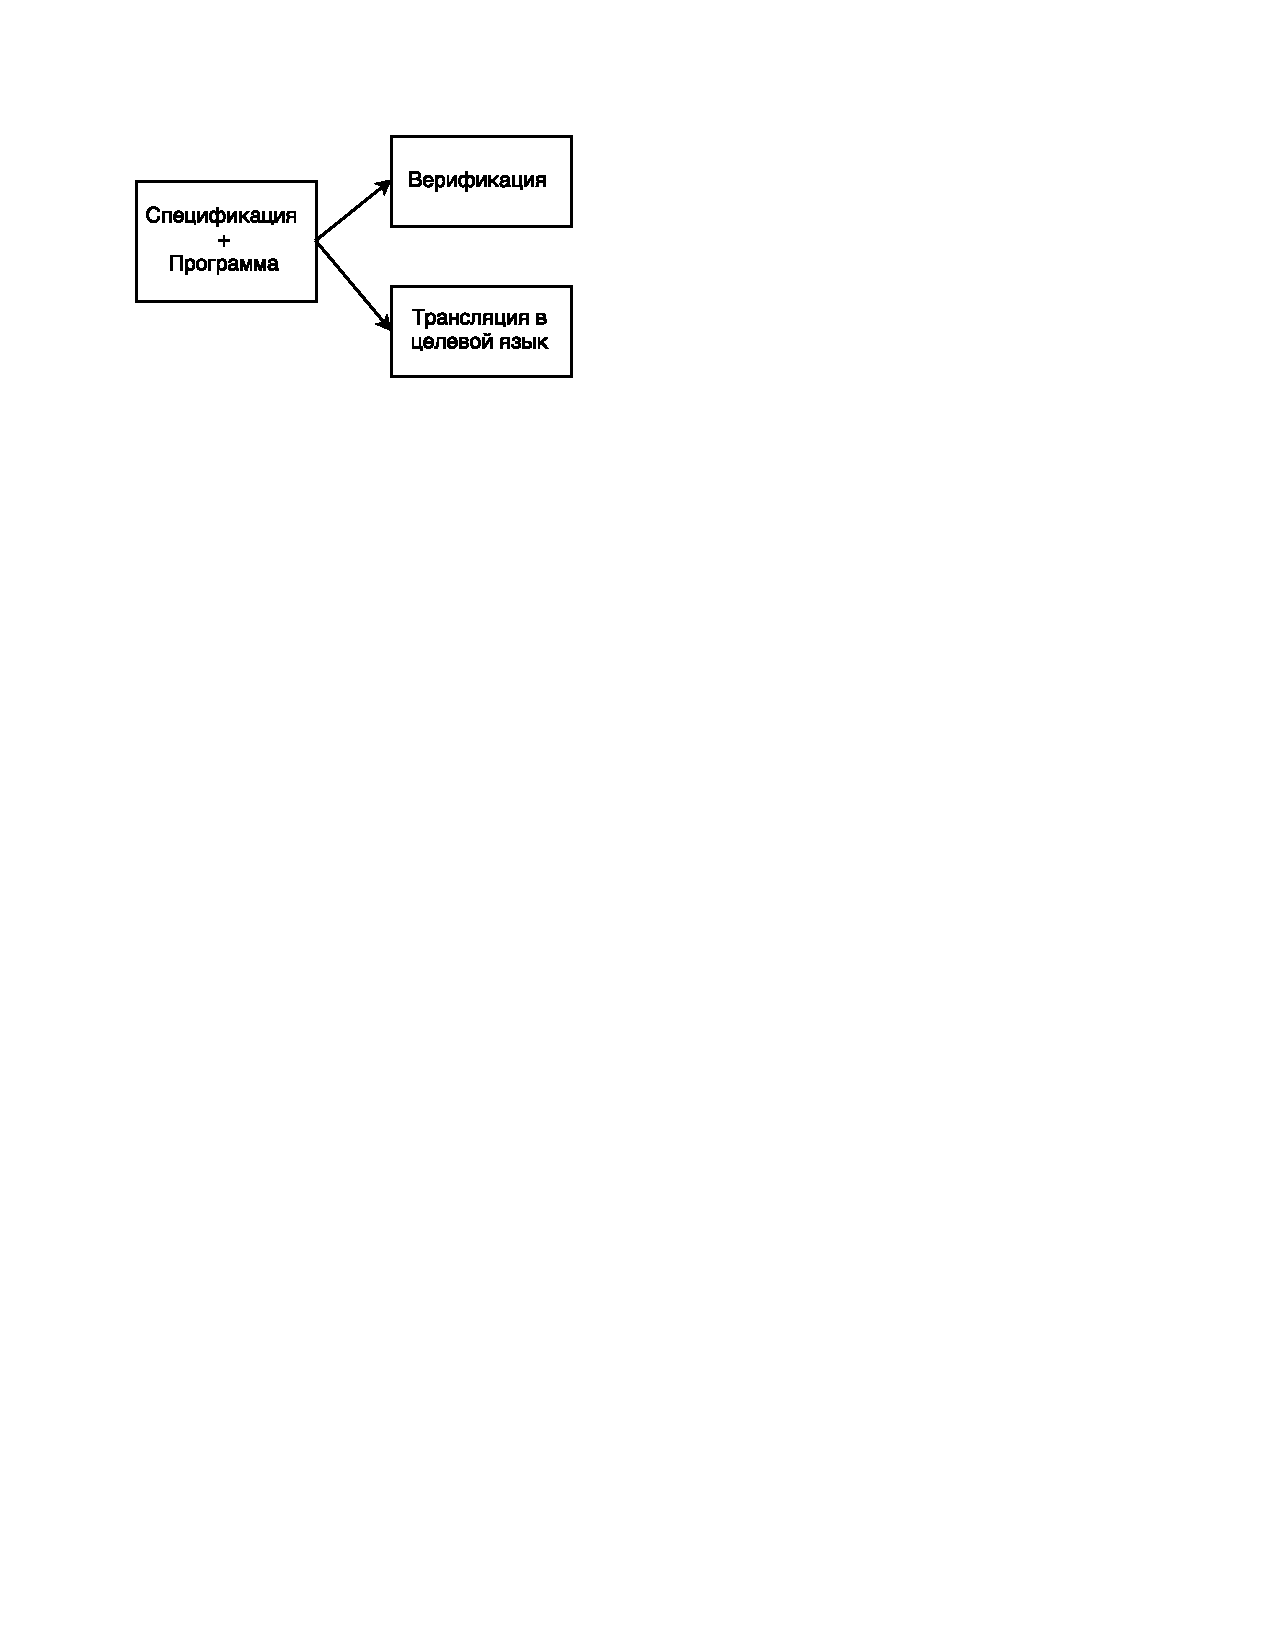
\includegraphics[width=.4\linewidth]{CertPr}}
\end{center}

\begin{itemize}
\item Позволяет доказывать, что программа соответствует своему формальному описанию
\item Инструменты для создания сертифицированных программ
	\begin{itemize}
	\item Coq, Agda, F*, Idris и др.
\end{itemize}
\end{itemize}

\end{frame}

\begin{frame}
\transwipe[direction=90]
\frametitle{Проект Everest}

Целью проекта является создание высокопроизводительной, соответствующей спецификациям, реализации протокола HTTPS

\begin{itemize}
\item Проект miTLS посвящен верификации протокола TLS
\item Проект HACL* посвящен верификации криптографических примитивов
\item Язык программирования F*, ориентированный на верификацию программ
\item KreMLin --- компилятор из подмножества языка F* в C
\item Язык программирования Vale и инструмент Dafny для создания и верификации криптографических примитивов на ассемблере
\end{itemize}

\end{frame}

\begin{frame}
\transwipe[direction=90]
\frametitle{Язык F*}

\begin{itemize}
\item Функциональный язык программирования, ориентированный на верификацию программ
\item Обладает богатой системой типов
	\begin{itemize}
	\item Уточняющие и зависимые типы
	\item Эффект вычисления функции и т.д.
	\end{itemize}
\item Позволяет доказывать многие свойства программы
\item \textbf{F* backends}
	\begin{itemize}
	\item OCaml
	\item C* $\to$ KreMLin $\to$ C
	\end{itemize}
\end{itemize}

\end{frame}

\begin{frame}
\transwipe[direction=90]
\frametitle{Существующие инструменты для компиляции программ на OCaml в JavaScript}

\begin{itemize}
\item js\_of\_ocaml
	\begin{itemize}
	\item Компиляция происходит на уровне байт-кода
	\item Не предназначен для чтения сгенерированного кода 
	\item Многие OCaml-библиотеки содержат вставки кода на C
	\end{itemize}
\item BuckleScript
	\begin{itemize}
	\item Компиляция происходит на уровне лямбда-выражений
	\item Читабельность сгенерированного кода
	\item Использование внутреннего представления для некоторых структур данных
	\end{itemize}	
\end{itemize}

\end{frame}


\begin{frame}
\transwipe[direction=90]
\frametitle{Инструмент Flow}
\begin{itemize}
\item Инструмент для статической проверки типов в JavaScript-\\программах
\item Поддержана спецификация ECMAScript 6
\item Почему не язык программирования TypeScript?
	\begin{itemize}
	\item Flow имеет более точную и богатую систему типов, чем TypeScript
	\item Для Flow: аннотация типов легко убирается из программы
	\item Логика работы системы типов Flow близка к той, что используется в функциональных языках программирования
	\end{itemize}			
\end{itemize}
\end{frame}


\begin{frame}
\transwipe[direction=90]
\frametitle{Постановка задачи}

\textbf{Цель:} разработать инструмент для компиляции сертифицированных F*-программ в робастные Веб-приложения на JavaScript

\begin{itemize}
\item Сформулировать правила трансляции с языка F* на JavaScript, гарантирующие сохранение аннотаций типов
\item Выполнить реализацию предложенного подхода
\item Провести экспериментальное исследование реализованного инструмента
\end{itemize}
\end{frame}


\begin{frame}
\transwipe[direction=90]
\frametitle{Описание подхода}

\begin{center}
.fst $\xrightarrow[]{~1~}$ F* AST  $\xrightarrow[]{~2~}$ ML AST $\xrightarrow[]{~3~}$ Flow AST $\xrightarrow[]{~4~}$ .flow $\xrightarrow[]{~5~}$ .js
\end{center}

\begin{itemize}
\item \textbf{Шаг 1:} построение F* AST исходной программы
\item \textbf{Шаг 2:} построение ML AST из F* AST (удаление зависимых и уточняющих типов, ghost-вычислений)
\item \textbf{Шаг 3:} трансляция ML AST в Flow AST с сохранением аннотаций для типов
\item \textbf{Шаг 4:} получение программы, которая может быть проверена инструментом Flow
\item \textbf{Шаг 5:} преобразование Flow-программы в JavaScript-программу (удаляется информация о типах)
\end{itemize}
    
\end{frame}

\begin{frame}
\transwipe[direction=90]
\frametitle{Правила трансляции языка OCaml в JavaScript}

Сформулированы правила трансляции для подмножества языка OCaml в JavaScript
\begin{itemize}
\item Константы
\item Выражения
\item Выражения для сопоставления с образцом
\item Типы
\end{itemize}

\end{frame}


\begin{frame}
\transwipe[direction=90]
\frametitle{Архитектура инструмента}

\begin{center}
   {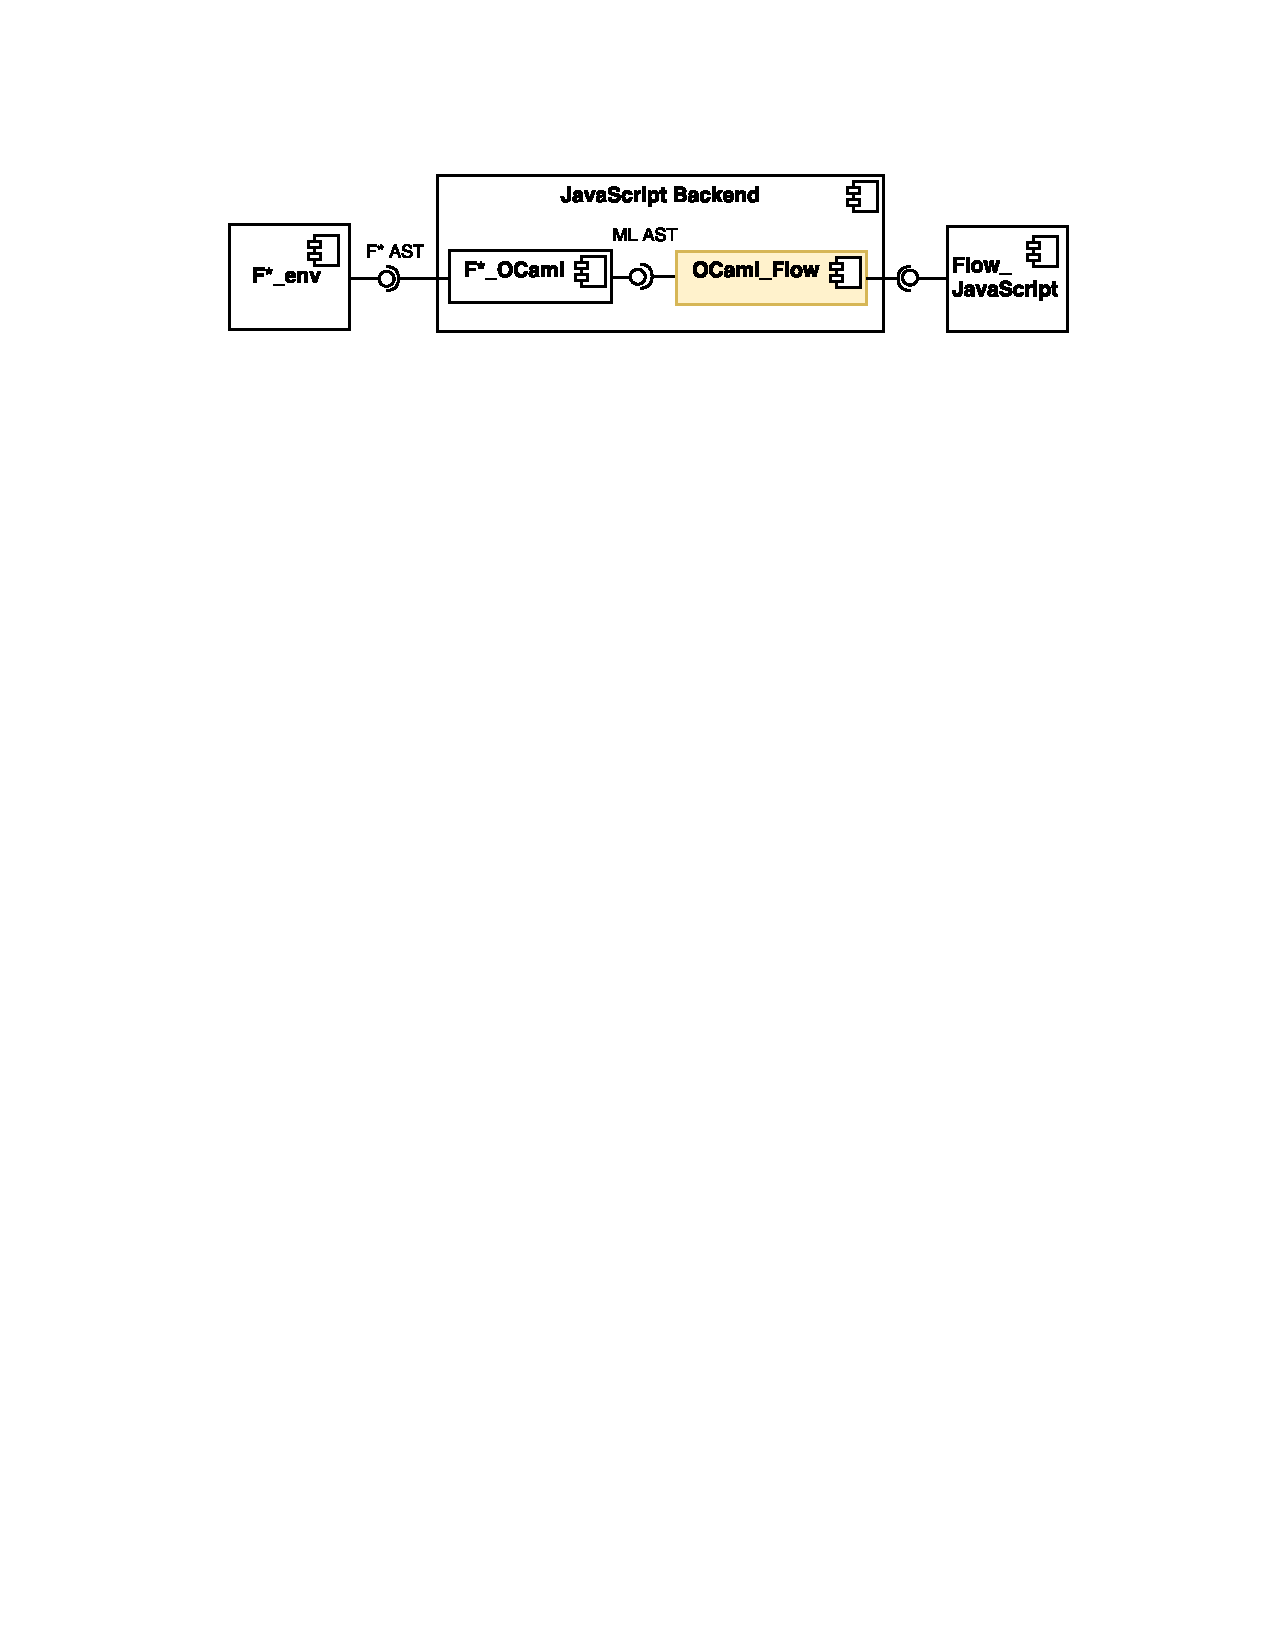
\includegraphics[width=.9\linewidth]{DiagComp}}
\end{center}

\end{frame}

\begin{frame}
\transwipe[direction=90]
\frametitle{Процесс построения JavaScript-приложения из F*-программы}

\begin{center}
   {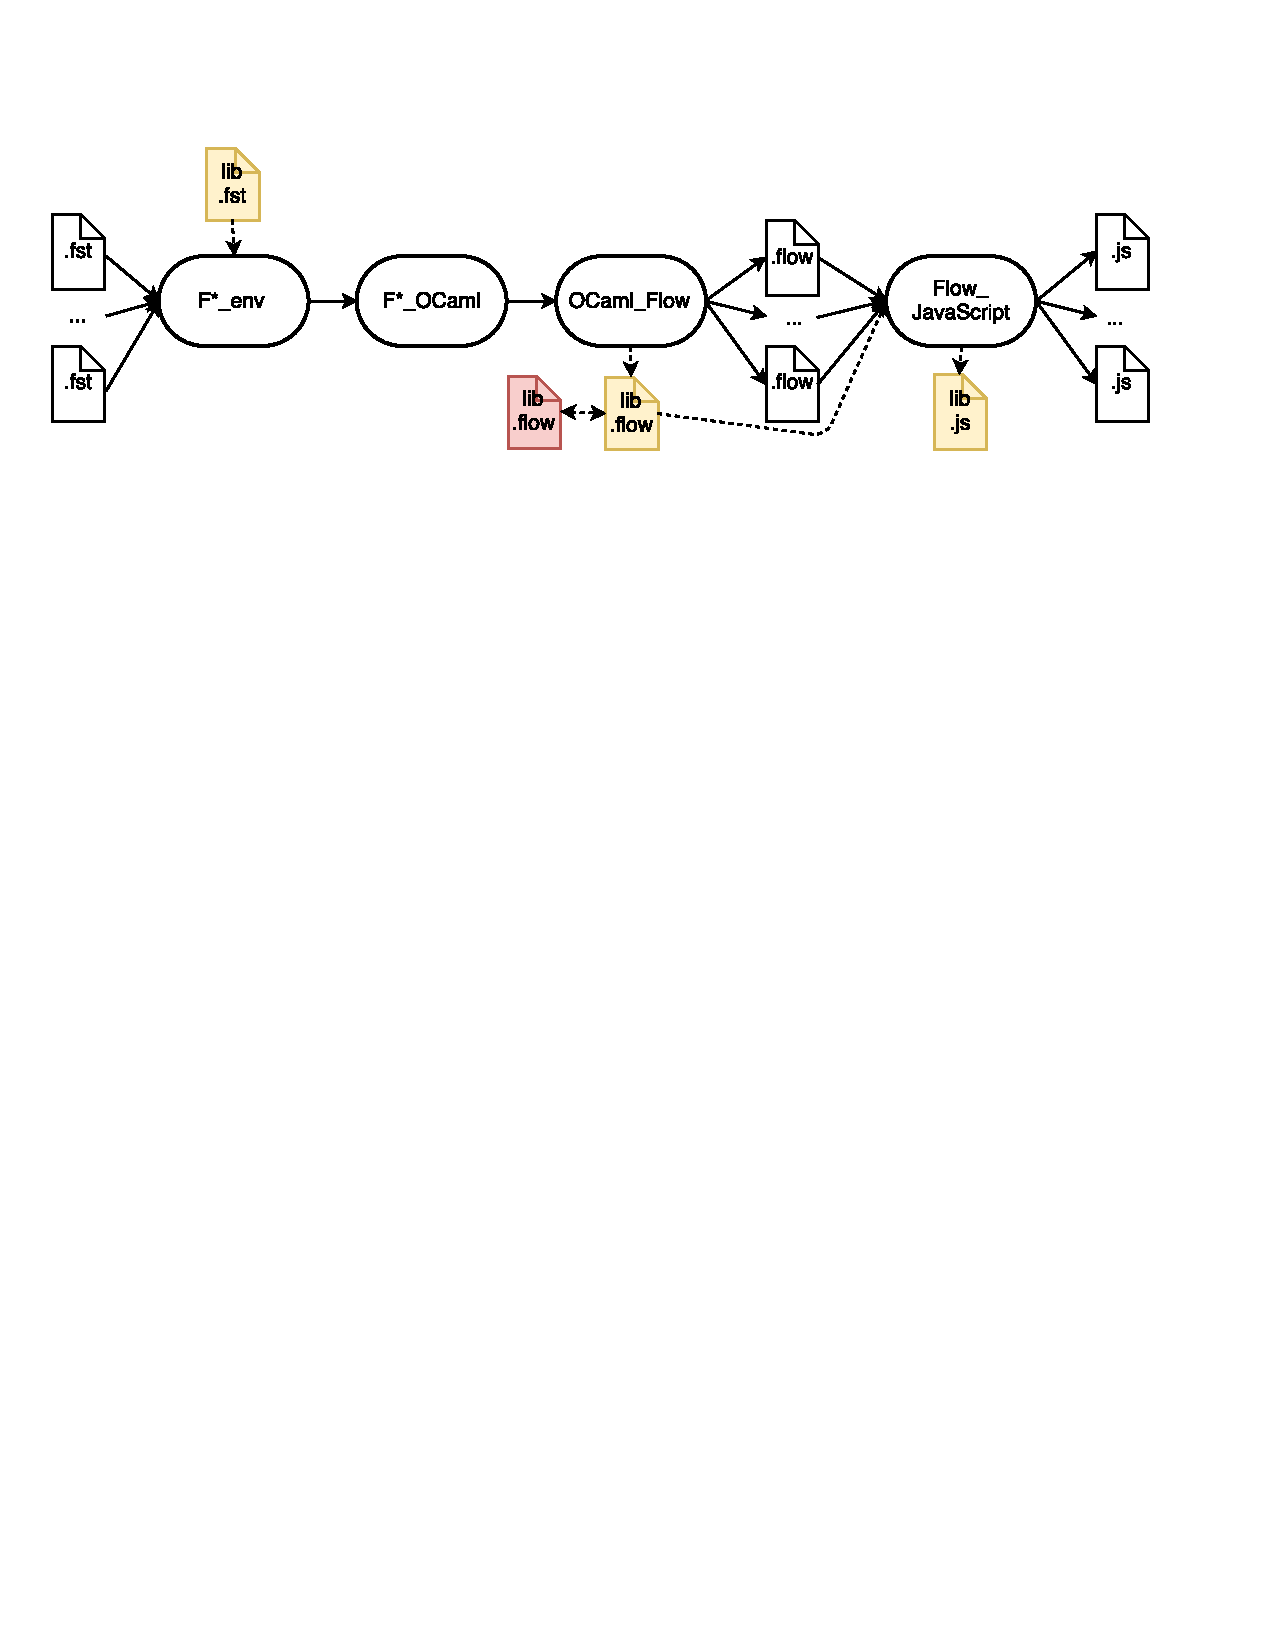
\includegraphics[width=1.0\linewidth]{Workflow}}
\end{center}

\end{frame}


\begin{frame}
\transwipe[direction=90]
\frametitle{Экспериментальное исследование}

\begin{itemize}
\item Тестовые данные: реализация алгоритма ChaCha20 из библиотеки HACL*
\item Для верификации алгоритма использовалось около 37 библиотечных и вспомогательных модулей

\item Описательная характеристика основного модуля
\begin{tabular}{ | c | c | c | c | }
\hline
& F* & F*\_OCaml & F*\_Flow \\ \hline
Кол-во верхнеуровневых функций & 32 & 32 & 32 \\ \hline
Кол-во строк кода & 786 & 422 & 316 \\
\hline
\end{tabular}

\item Выполнялись замеры времени работы функции 

\texttt{\textit{encrypt} plaintext key nonce counter $\to$ cyphertext}

\end{itemize}

\end{frame}

\begin{frame}
\transwipe[direction=90]
\frametitle{График сравнения времени выполнения программ}

\begin{center}
 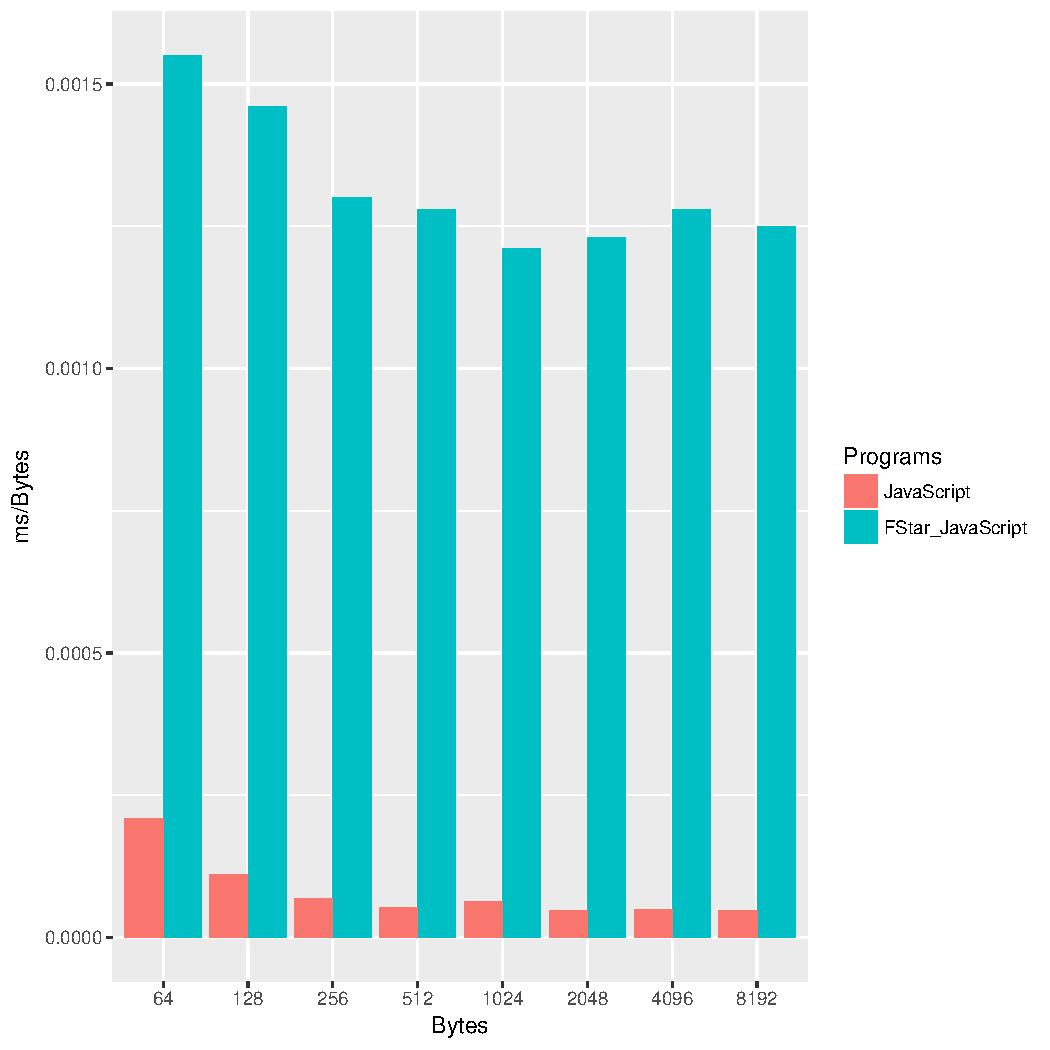
\includegraphics[width=.65\linewidth]{Comparison}
\end{center}

\end{frame}


\begin{frame}
\transwipe[direction=90]
\frametitle{Результаты}

\begin{itemize}
\item Сформулированы правила трансляции с языка F* на JavaScript
\item Выполнена реализация предложенного подхода на языке F*
\item Проведено экспериментальное исследование реализованного инструмента на примерах из криптографической библиотеки HACL*
\end{itemize}
\end{frame}

\end{document}
